\section{Introduction}
\label{section:p450/introduction}
The most common method of drug clearance among currently perscribed drugs is metabolism, which is the primary method of clearance for approximately 75\% of the top 200 most commonly perscribed drugs in the United States \cite{williams2004drug}.
Cytochrome p450 is critical to drug metabolism, being active in approximately 75\% of drugs which are cleared in this method \cite{guengerich2007cytochrome}. 
As covered in \ref{subsubsection:lead_optimization}, accurately predicting  absorption, distribution, metabolism, and excretion, characteristics of drug compounds can be a critical determining factor in determining drug efficacy, performance in clinical development stages, and the overall costs of bringing new drugs to market.
Because of the ubiquity of P450 in metabolic reactions of drugs, there is no other single enzyme family as significant to determining ADME as P450.   

\begin{figure}[h]
\centering
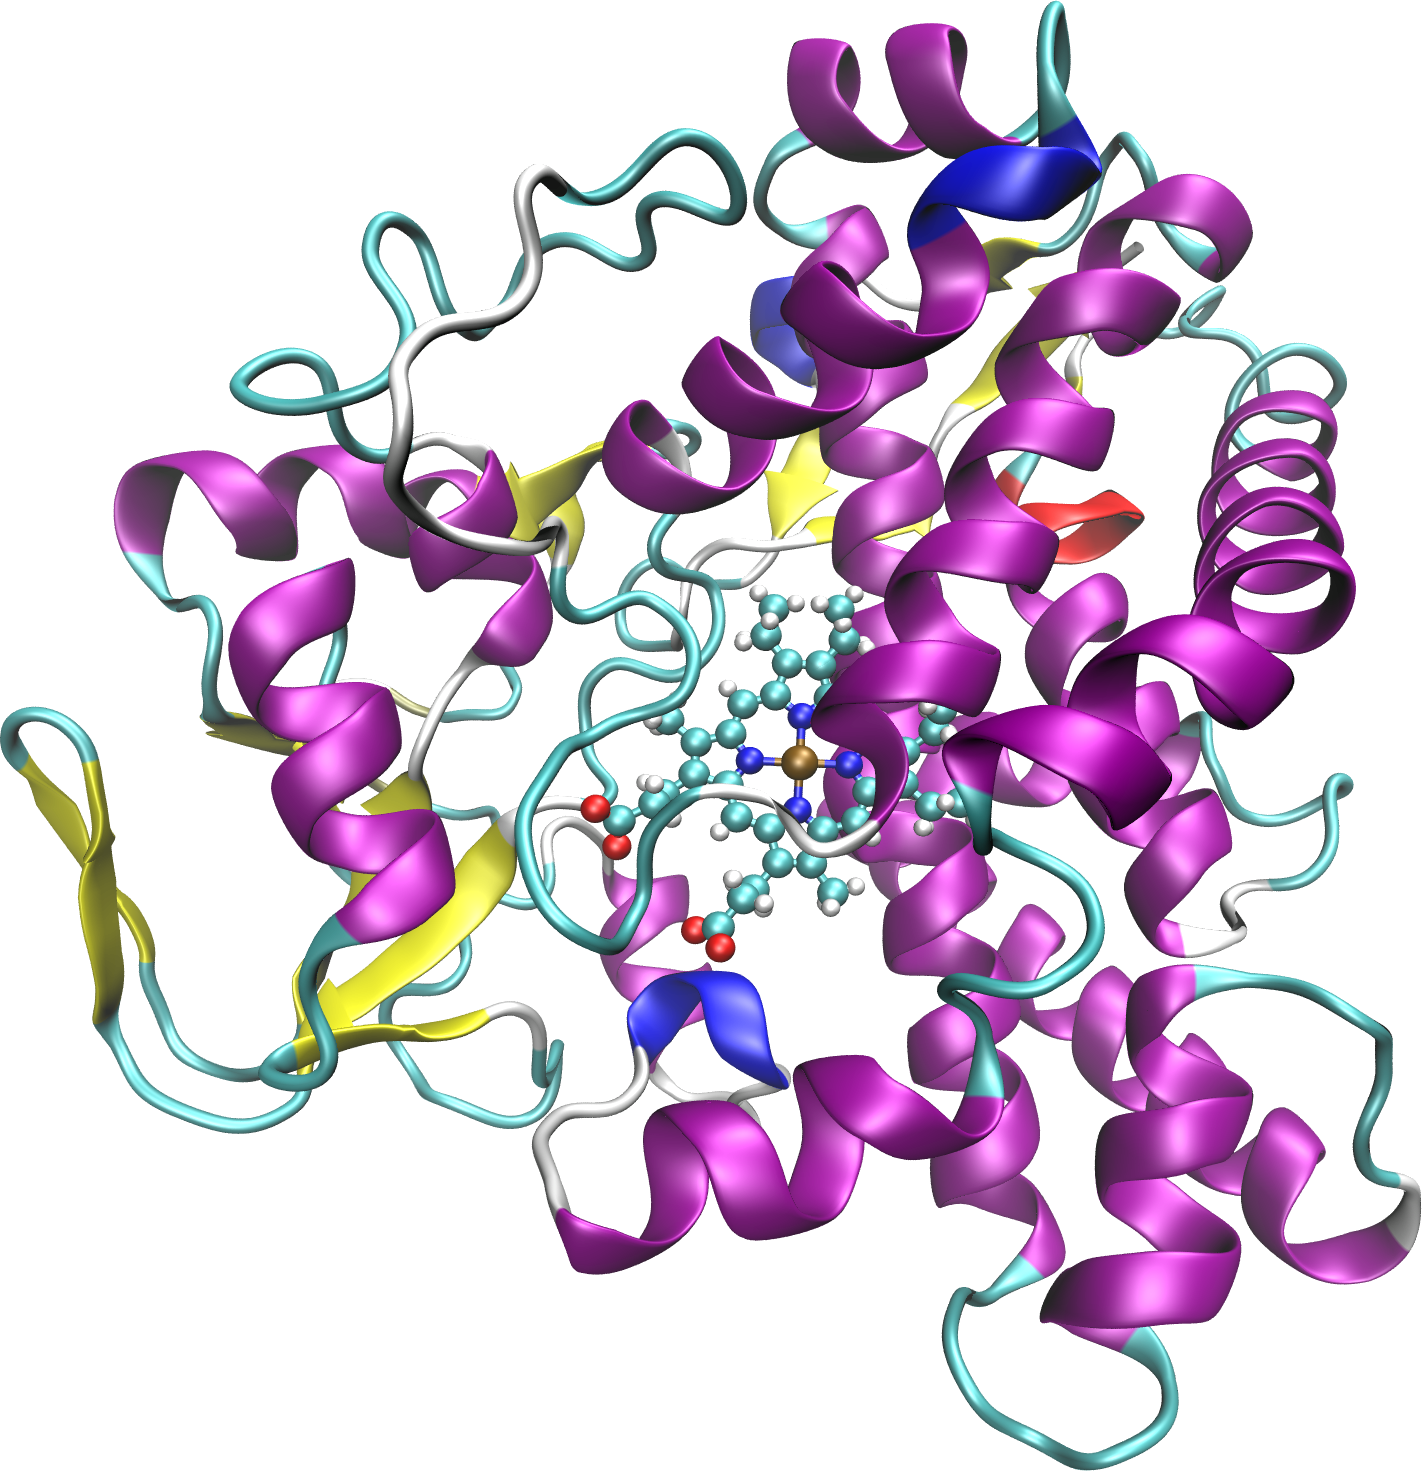
\includegraphics[width=0.5\textwidth]{figures/p450.png}
\caption{
The structure of cytochrome P450, taken from PDBid 1JFB, shown in cartoon representation.
The bonded heme group, shown as ball and stick model, is visible in the center.
}
\label{fig:p450}
\end{figure}

